\documentclass[12pt,a4paper]{report}

\usepackage[T1]{fontenc}
\usepackage[utf8]{inputenc}
\usepackage{newtxtext,newtxmath}
\usepackage{setspace}
\usepackage[left=1.2in,right=0.8in,top=1in,bottom=1.25in]{geometry}
\usepackage{graphicx}
\usepackage{booktabs}
\usepackage{array}
\usepackage{longtable}
\usepackage{tabularx}
\usepackage{url}
\usepackage{hyperref}
\usepackage{enumitem}
\usepackage{titlesec}
\usepackage{caption}
\usepackage{float}
\usepackage{cite}

\onehalfspacing
\setlength{\parindent}{12mm}
\setlength{\parskip}{0.4em}

\titleformat{\chapter}[display]
  {\bfseries\centering\fontsize{18}{20}\selectfont}
  {Chapter \thechapter}
  {18pt}
  {}

% Reduce extra vertical whitespace above chapter headings.
\titlespacing*{\chapter}{0pt}{0pt}{12pt}

\captionsetup[table]{position=top}
\captionsetup[figure]{position=bottom}

\newcommand{\projecttitle}{Data Centric Approach to Train Delay Prediction in Indian Railways}
\newcommand{\deptname}{Department of Artificial Intelligence and Data Science}
\newcommand{\institutename}{Samrat Ashok Technological Institute, Vidisha}
\newcommand{\sessionname}{Session 2026}
\newcommand{\submissionmonth}{May 2026}

\begin{document}

% -------------------------
% Cover Page
% -------------------------
\begin{titlepage}
\centering
\vspace*{1.5cm}
{\Large \textbf{MINOR PROJECT REPORT}}\\[1.2cm]
{\LARGE \textbf{\projecttitle}}\\[1.5cm]

\textit{Submitted in partial fulfillment of the requirements for the award of the degree of}\\[0.3cm]
{\large \textbf{Bachelor of Technology}}\\[0.2cm]
{\large in}\\[0.2cm]
{\large \textbf{Artificial Intelligence and Data Science}}\\[1.2cm]

\textbf{Submitted by}\\[0.5cm]
\begin{tabular}{ll}
Arjun Sarje & 0108AI231020 \\
Ashvin Sukaye & 0108AI231023 \\
Vyomesh Khare & 0108AI231077 \\
\end{tabular}

\vfill
\textbf{Under the Guidance of}\\[0.2cm]
Prof. Rashi Kumar\\[1.0cm]

\textbf{\deptname}\\
\textbf{\institutename}\\
\textbf{\sessionname}\\
\textbf{\submissionmonth}
\end{titlepage}

% Front matter page numbering (i, ii, iii, ...)
\pagenumbering{roman}

% -------------------------
% Declaration (2nd printed page)
% -------------------------
\chapter*{Declaration}
\addcontentsline{toc}{chapter}{Declaration}
We hereby declare that the work presented in this minor project report entitled \textit{\projecttitle} is the original work carried out by us under the guidance of Prof. Rashi Kumar, \deptname, \institutename.

This work has not been submitted, either in full or in part, for the award of any degree or diploma to any other university or institution. We further declare that all sources of information used in this report have been appropriately acknowledged and cited.

We understand that in case any violation of academic ethics or plagiarism is found, we shall be solely responsible for the same.

\vspace{1.5cm}
\begin{tabular}{p{0.55\textwidth}p{0.35\textwidth}}
Arjun Sarje (0108AI231020) & Date: \hrulefill \\
Ashvin Sukaye (0108AI231023) & Date: \hrulefill \\
Vyomesh Khare (0108AI231077) & Date: \hrulefill \\
\end{tabular}

\clearpage

% -------------------------
% Acknowledgment
% -------------------------
\chapter*{Acknowledgment}
\addcontentsline{toc}{chapter}{Acknowledgment}
We express our sincere gratitude to our project guide, Prof. Rashi Kumar, for her valuable guidance, continuous support, and constructive feedback throughout this project.

We are thankful to the Project Coordinator for systematic coordination and timely academic support during the minor project phase.

We respectfully acknowledge the Head of the Department of AI\&DS, Prof. Sunil Joshi sir, for his encouragement and guidance. We also extend our sincere thanks to the Director sir of \institutename{} for providing institutional support and opportunities for academic growth.

We are grateful to all teaching and non-teaching staff members of the Department of AI\&DS for their assistance and cooperation.

Finally, we thank our peers and families for their continuous motivation and support.

\clearpage

% -------------------------
% Thesis Certificate (4th printed page)
% -------------------------
\chapter*{Thesis Certificate}
\addcontentsline{toc}{chapter}{Thesis Certificate}
This is to certify that the minor project report entitled \textit{\projecttitle} submitted by:
\begin{itemize}[leftmargin=2em]
    \item Arjun Sarje (0108AI231020)
    \item Ashvin Sukaye (0108AI231023)
    \item Vyomesh Khare (0108AI231077)
\end{itemize}
is a bona fide record of work carried out by them under my supervision in partial fulfillment of the requirements for the award of the degree of Bachelor of Technology in Artificial Intelligence and Data Science during \sessionname.

\vspace{2cm}
\begin{tabular}{>{\centering\arraybackslash}p{0.45\textwidth}>{\centering\arraybackslash}p{0.45\textwidth}}
Guide Signature & Head of Department Signature \\
Prof. Rashi Kumar & \deptname \\
\end{tabular}

\vspace{1.2cm}
\noindent Place: Vidisha\\
Date: \hrulefill

\clearpage

% -------------------------
% Abstract
% -------------------------
\chapter*{Abstract}
\addcontentsline{toc}{chapter}{Abstract}
Indian Railways delay analytics faces a critical data bottleneck: there is no widely available, open, station-level, machine-learning-ready real-time dataset for longitudinal modeling of delay propagation. This project addresses the gap through a data-centric approach that prioritizes robust data engineering before advanced prediction.

We designed and deployed an automated collection pipeline using GitHub Actions cron workflows, RailRadar API polling, and Supabase PostgreSQL persistence. The system tracks journey lifecycle states and stores station-level scheduled/actual timestamps and delay fields through an idempotent, fault-aware architecture. Since January 2026, the pipeline has been running continuously for a fixed train panel (10 trains, including both single-day and multi-day services), and by late April 2026 the system has collected more than 40,000 unique station-level records.

After data collection, we performed exploratory data analysis and preprocessing to standardize timestamps, route ordering, and journey-wise comparisons. Train-wise plots of station vs departure delay over 30-day windows showed recurring operational patterns: some station segments tend to consistently add delay, while others consistently recover delay. To quantify this behavior, we formulated a station-pair delay-delta indicator (alpha), computed over adjacent halt stations. Median alpha values were used to classify route segments into delay-adding, neutral, and delay-cover-up zones, supporting interpretable operational diagnosis.

We also developed baseline prediction experiments for next-station delay using classical machine learning and time-series models. Initial results provide a benchmark, but current performance is not yet sufficient to capture all learned route-level patterns. The next phase focuses on improved preprocessing, normalization, richer feature engineering, and advanced approaches such as graph-structured embeddings for station network behavior.

The project outcome is both a usable dataset-generation infrastructure and an analysis framework that can support future delay prediction research specific to Indian Railways.

\clearpage

% Front matter lists
\tableofcontents
\clearpage
\listoffigures
\clearpage
\listoftables
\clearpage

\chapter*{List of Abbreviations and Nomenclature}
\addcontentsline{toc}{chapter}{List of Abbreviations and Nomenclature}
\begin{longtable}{p{0.28\textwidth}p{0.62\textwidth}}
API & Application Programming Interface \\
EDA & Exploratory Data Analysis \\
ETL & Extract Transform Load \\
IST & Indian Standard Time \\
ML & Machine Learning \\
RF & Random Forest \\
ARIMA & AutoRegressive Integrated Moving Average \\
SARIMA & Seasonal ARIMA \\
DB & Database \\
alpha & Station-pair delay delta indicator used in this report \\
\end{longtable}

\clearpage
\pagenumbering{arabic}

% -------------------------
% CHAPTER 1
% -------------------------
\chapter{Introduction}

\section{Background and Need}
Indian Railways operates at very large scale and is sensitive to delay propagation across stations and routes. Despite this scale, public, station-level, real-time datasets suitable for reproducible delay analytics are limited. Existing studies are often constrained by survey-based data, short observation windows, or inaccessible proprietary sources.

This makes model development difficult because delay prediction quality depends heavily on consistent and long-duration data with journey context. Therefore, this project started with a data-centric goal: build a reliable automated pipeline first, then use the collected dataset for analytics and modeling.

\section{Project Motivation}
During initial planning and literature review, we found that open resources for Indian Railways delay modeling are sparse compared to international systems. This motivated us to design our own data pipeline and to publish methodology and evidence. The first phase of this work was presented in Technovision 2026 (paper presentation competition on standards at SATI, Vidisha) and received first prize in the AI\&DS domain.

\section{Objectives}
The key objectives of this minor project are:
\begin{enumerate}
    \item Build a scalable, automated, reproducible pipeline to collect station-level delay data for selected trains.
    \item Maintain journey lifecycle tracking to preserve completion and failure context.
    \item Perform train-wise exploratory analysis to identify persistent delay patterns.
    \item Quantify station-segment behavior using a robust route-level metric (alpha).
    \item Establish baseline delay prediction models as a reference for future improvements.
\end{enumerate}

\section{Contributions in Current Phase}
\begin{itemize}
    \item Continuous collection pipeline operational since January 2026.
    \item More than 40,000 unique station-level records collected as of late April 2026.
    \item EDA workflow for 10 trains with halt-station aligned trend plots.
    \item Station-pair alpha analysis for identifying delay-add and delay-recovery zones.
    \item Baseline prediction experiments (Random Forest, Polynomial Regression, and time-series trials such as ARIMA, SARIMA, Prophet, and Chronos).
\end{itemize}

\section{Organization of the Report}
The report is organized as follows: Chapter 2 reviews literature and identifies research gaps. Chapter 3 formalizes the problem statement. Chapter 4 describes the proposed and implemented system architecture and methodology. Chapter 5 presents dataset statistics, analysis results, alpha findings, and baseline modeling outcomes. Chapter 6 concludes the current work and outlines future directions.

% -------------------------
% CHAPTER 2
% -------------------------
\chapter{Fundamentals and Literature Survey (Theory)}

\section{Railway Delay Modeling in International Context}
International railway systems such as those in the UK and Germany provide open operational feeds that support reproducible analytics \cite{uk_rail_data,german_rail_data}. Prior studies have applied machine learning and propagation models for delay forecasting and traffic optimization \cite{oneto2018train,flier2009delay,goverde2010railway}. These datasets typically include structured temporal events and multi-year coverage.

\section{Indian Context and Data Availability Gap}
For Indian Railways, there has been meaningful research on delay prediction, but reproducible open data access remains limited. Gaurav and Srivastava proposed a zero-shot Markov framework using data from 135 trains over March 2016 to February 2018, yet the underlying dataset/source is not openly released for direct reproduction \cite{gaurav2018zeroshot}. Arshad also reported machine learning based delay prediction with data references to online running status sources, but without an openly shareable benchmark dataset in the publication workflow \cite{arshad2019prediction}. More recently, RSTGCN reports a nationwide Indian railway delay dataset claim, but at present the dataset is not publicly accessible through links in the paper/repository trail, which limits independent verification and reuse \cite{chowdhury2025rstgcn}. While high-level reports exist \cite{indian_railways_stats}, model-ready station-level traces with continuous open access are still uncommon.

\section{Fundamentals Used in This Work}
\subsection{Delay Variables}
Two primary variables are used in our dataset: delay at arrival and delay at departure (in minutes). These are combined with scheduled and actual timestamps at each station to analyze accumulation/recovery behavior.

\subsection{Journey Lifecycle Tracking}
Instead of only collecting raw snapshots, we track journey state with explicit completion and abandonment flags. This enables controlled extraction and reduces duplication.

\subsection{Station-Sequence Analysis}
Route analysis is performed on halt-only station order to provide consistent sequence alignment across journey dates, allowing segment-level comparisons.

\section{Comparative Literature Insight}
Most prior work emphasizes prediction models; however, prediction quality is strongly data-dependent. In our case, delay forecasting was the intended primary objective, but lack of consistently accessible dataset infrastructure became an enabling bottleneck that had to be solved first. This project therefore contributes a data-first pipeline for Indian context and introduces an interpretable station-pair alpha indicator for operational insight prior to stronger model claims.

\section{End-of-Chapter Synthesis}
The literature indicates that data quality, consistency, and operational context are prerequisites for robust prediction. Therefore, this phase prioritizes systematic data generation and station-level interpretability as a prerequisite stage, with forecasting performance improvement as the downstream target.

% -------------------------
% CHAPTER 3
% -------------------------
\chapter{Problem Statement}

\section{Core Problem}
The primary long-term problem is robust train delay forecasting for Indian Railways, especially station-to-station delay propagation and arrival-time reliability improvement. However, in practical execution we found an enabling problem first: absence of sufficiently open, continuously collected, station-level data needed to train and validate such models.

\section{Observed Challenges}
\begin{itemize}
    \item Missing open historical traces with journey-state context.
    \item Sparse reproducible pipelines publicly documented for Indian routes.
    \item Difficulty in comparing station behavior across journey dates without stable ordering.
    \item Baseline models struggle without route-aware feature design and normalized preprocessing.
    \item Existing public-facing ETA systems are often perceived as heavily timetable/heuristic driven, motivating a stronger data-driven alternative for delay-aware predictions.
\end{itemize}

\section{Formal Project Problem Statement}
Design and operate an automated data pipeline that collects reliable station-level delay data for selected Indian trains, then develop a data analysis framework that can:
\begin{enumerate}
    \item reveal persistent station-segment delay behavior,
    \item quantify delay accumulation/recovery zones,
    \item and provide benchmark delay-forecasting baselines for future model enhancement.
\end{enumerate}

\section{How Proposed Work Addresses Existing Schemes}
Unlike approaches that begin directly from model training on limited snapshots, this work first constructs a reproducible data foundation with lifecycle tracking, idempotent storage, and explicit quality checks. This directly addresses the enabling bottleneck (data availability) so that the primary objective (better delay forecasting) can be pursued with stronger evidence in subsequent phases.

% -------------------------
% CHAPTER 4
% -------------------------
\chapter{Proposed Work}

\section{System Overview}
The implemented system uses a serverless execution model driven by scheduled workflows and cloud database storage. Two polling workflows are maintained: one for one-day trains and one for multi-day trains.

\begin{figure}[H]
\centering
\IfFileExists{../system_architecture.png}{
    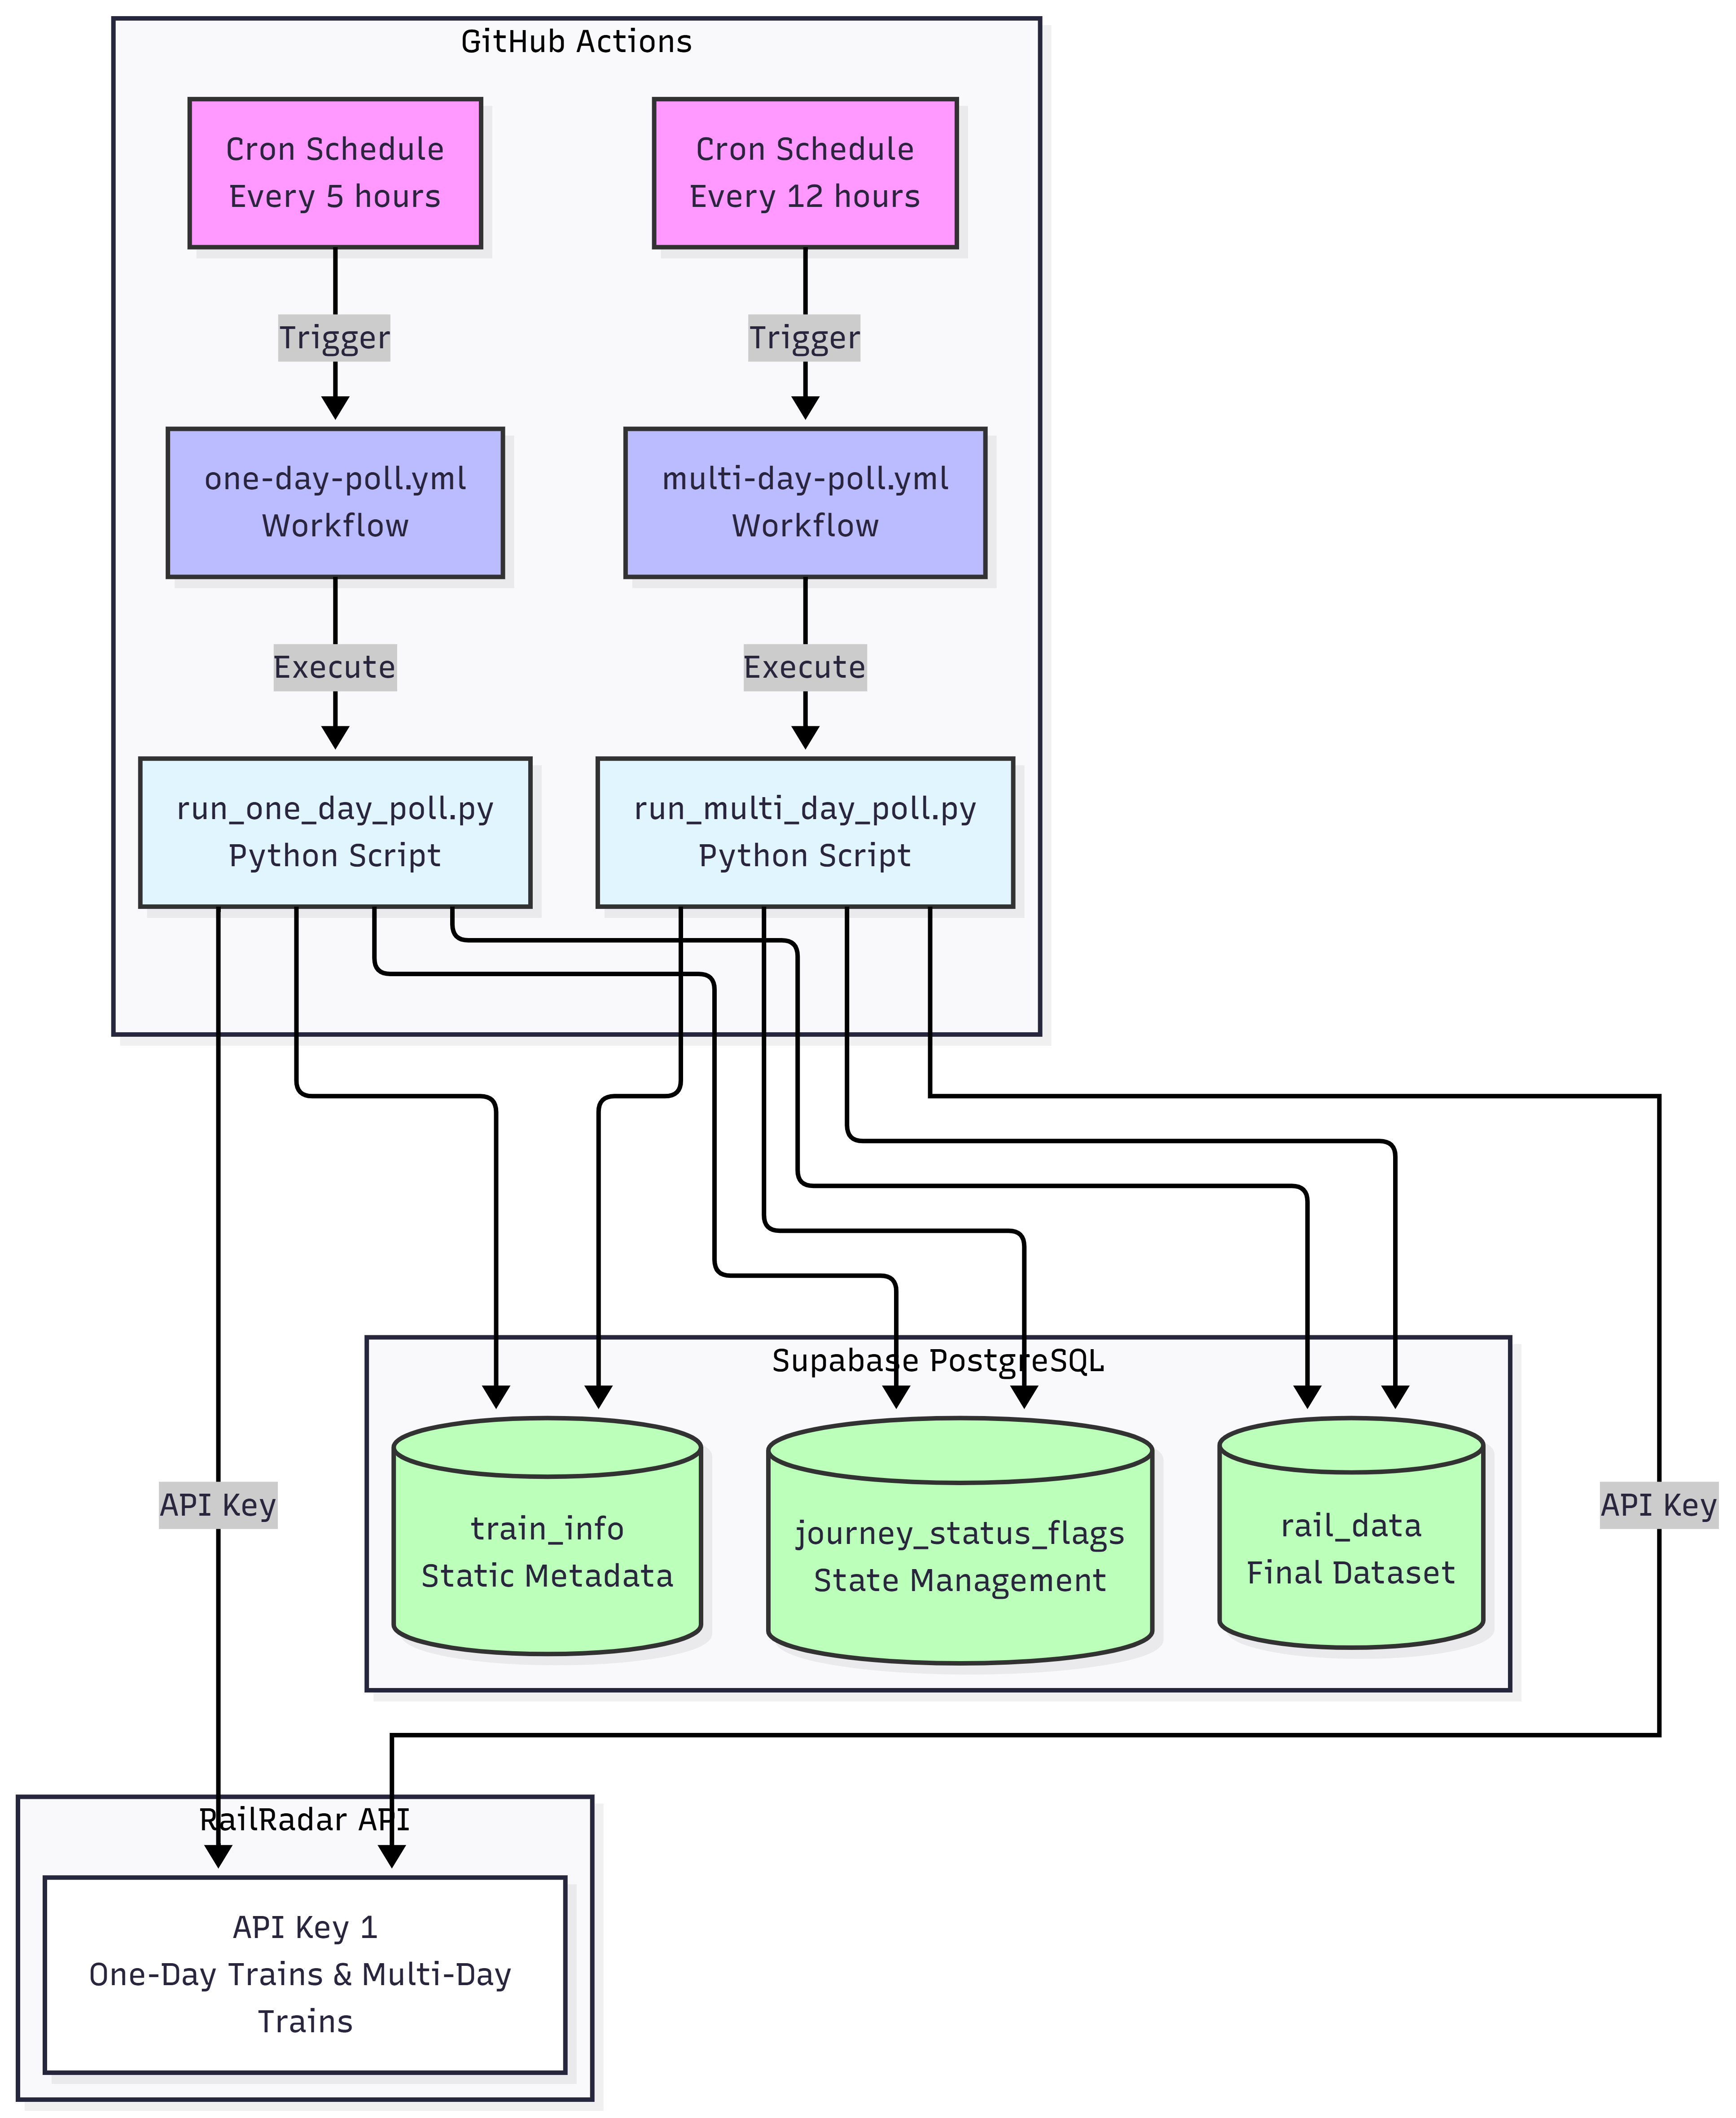
\includegraphics[width=0.75\textwidth]{../system_architecture.png}
}{
    \fbox{\parbox{0.9\textwidth}{Placeholder: system architecture diagram}}
}
\caption{Automated data collection architecture integrating scheduler, API, and database.}
\label{fig:arch}
\end{figure}

\section{Dual-Phase Polling Methodology}
\subsection{Phase 1: New Journey Detection}
For each configured train, the pipeline checks whether a journey record already exists for the current IST date. If not, RailRadar live data is queried to confirm journey start conditions. On valid start, a new tracker row is inserted with initial flag values.

\subsection{Phase 2: Ongoing Journey Tracking}
All journeys marked neither completed nor abandoned are polled. Completion is detected when current station code matches configured destination code. On completion, route station records are inserted into the main dataset table. On repeated failures, flag counters increase and eventually trigger abandonment.

\begin{figure}[H]
\centering
\IfFileExists{../journey_state_diagram.png}{
    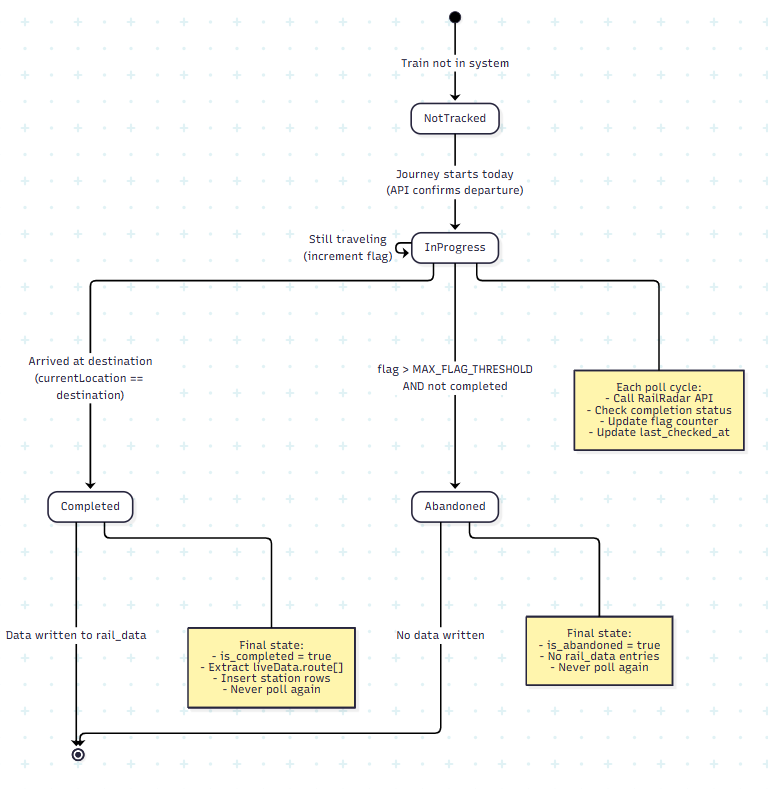
\includegraphics[width=0.75\textwidth]{../journey_state_diagram.png}
}{
    \fbox{\parbox{0.3\textwidth}{Placeholder: journey state machine diagram}}
}
\caption{Journey state machine used for robust lifecycle tracking.}
\label{fig:state_machine}
\end{figure}

\section{Database Design}
The data model consists of three connected tables.

\begin{table}[H]
\centering
\caption{Core database tables and roles}
\label{tab:db_schema}
\begin{tabular}{p{0.24\textwidth}p{0.68\textwidth}}
\toprule
Table & Purpose \\
\midrule
train\_info & Static metadata for monitored trains (name, journey type, destination). \\
journey\_status\_flags & Journey-level state tracking: completion, abandonment, and polling flag count. \\
rail\_data & Station-level observations with scheduled/actual times and delay fields. \\
\bottomrule
\end{tabular}
\end{table}

\subsection{Schema}
Table \ref{tab:schema_simple} summarizes the table-level schema in an easy-to-read format based on implemented migrations.

\begin{table}[H]
\centering
\caption{Database schema summary}
\label{tab:schema_simple}
\small
\begin{tabular}{p{0.22\textwidth}p{0.28\textwidth}p{0.42\textwidth}}
\toprule
Table & Key Fields & Important Columns \\
\midrule
train\_info & train\_no (unique) & train\_name, journey\_type (one\_day/multiple\_day), destination\_station\_code, journey\_duration \\
journey\_status\_flags & (train\_no, journey\_date) unique & flag, is\_completed, is\_abandoned, last\_checked\_at, created\_at, updated\_at \\
rail\_data & (train\_no, journey\_date, station\_code) unique & scheduled/actual arrival-departure timestamps, delay\_arrival\_minutes, delay\_departure\_minutes, distance\_from\_origin\_km \\
\bottomrule
\end{tabular}
\end{table}

\section{Reliability and Data Integrity}
\begin{itemize}
    \item Idempotent insertion policy avoids duplicate station rows.
    \item Composite keys maintain journey isolation for parallel journey handling.
    \item API failures are handled via controlled flag increments.
    \item Completion and insertion are logically tied to avoid inconsistent states.
\end{itemize}

\section{Train Panel and Collection Scope}
Ten representative trains were selected: 4 single-day services and 6 multi-day services, spanning short and long routes.

\begin{table}[H]
\centering
\caption{Monitored train panel used in current phase}
\label{tab:trains}
\begin{tabular}{cccc}
\toprule
Train No. & Train Name & Journey Type & Approx. Duration (h) \\
\midrule
61631 & Bhopal - Bina MEMU & one\_day & 3 \\
11605 & Bhopal - Bina MEMU Express & one\_day & 2 \\
11606 & Bina - Bhopal MEMU Express & one\_day & 2 \\
61632 & Bina - Bhopal MEMU & one\_day & 3 \\
12137 & Punjab Mail & multiple\_day & 33 \\
12138 & Punjab Mail & multiple\_day & 33 \\
11077 & Jhelum Express & multiple\_day & 40 \\
11078 & Jhelum Express & multiple\_day & 40 \\
18237 & Chhattisgarh Express & multiple\_day & 43 \\
18238 & Chhattisgarh Express & multiple\_day & 42 \\
\bottomrule
\end{tabular}
\end{table}

\section{Data Processing and EDA Workflow}
After establishing the collection pipeline, we executed a structured analysis phase in Python Jupyter notebooks. The workflow was performed in the following order:

\begin{enumerate}
    \item Initial statistical EDA and data quality checks: column profiling, datatype checks, missing-value ratios, and timestamp parse diagnostics.
    \item Time normalization and event-time construction: Unix timestamp conversion to IST and consistent journey-date processing for sequence analysis.
    \item Train-wise delay-curve visualization: station vs departure delay curves across journey windows using halt-station static ordering.
    \item Pattern discovery: visual identification that some station segments repeatedly add delay (upward trend) while others repeatedly cover up delay (downward trend).
    \item Baseline modeling: first benchmark models for delay forecasting (classical ML and time-series baselines).
    \item Segment-level experimentation on Train 18238: station-pair delta and alpha computation, followed by top-10 ranking outputs for delay-adding and recovery pairs.
\end{enumerate}

\subsection{From Visualization to Alpha Experimentation}
The alpha methodology was derived directly from the observed station-wise delay trend shapes. In the notebook, the experimentation block (cells 12--16 in the current notebook ordering) formalizes pairwise delay deltas, computes median/mean alpha, and reports ranked outputs (including top-10 delay-adding and top-10 recovery segments). This pipeline bridges exploratory visualization and interpretable operational analytics.

% -------------------------
% CHAPTER 5
% -------------------------
\chapter{Experimental Result Analysis}

\section{Dataset Snapshot and Preprocessing}
The collection system has been active since January 2026 and has crossed 40,000 unique station-level records by late April 2026. For analysis, timestamp fields were parsed and converted to IST; journey date and halt-station sequence were normalized for cross-journey comparison.

\subsection{Analyzed Fields}
Primary fields used in this phase include train number, journey date, station code, scheduled/actual arrival/departure timestamps, delay arrival/departure, and event-time derived ordering.

\section{Train-wise Delay Pattern Visualization}
For each train, a 30-day station vs departure-delay plot was generated in static route order (halt-only). Overlapping journey traces revealed that route behavior is not random: specific segments repeatedly show upward delay drift while others repeatedly reduce delay.

In the main chapter, we present Train 18238 (Chhattisgarh Express) as the representative experimentation case. Plots for the remaining nine trains are moved to Appendix II.

\begin{figure}[H]
\centering
\IfFileExists{../train_18238_station_delay_30d.png}{
    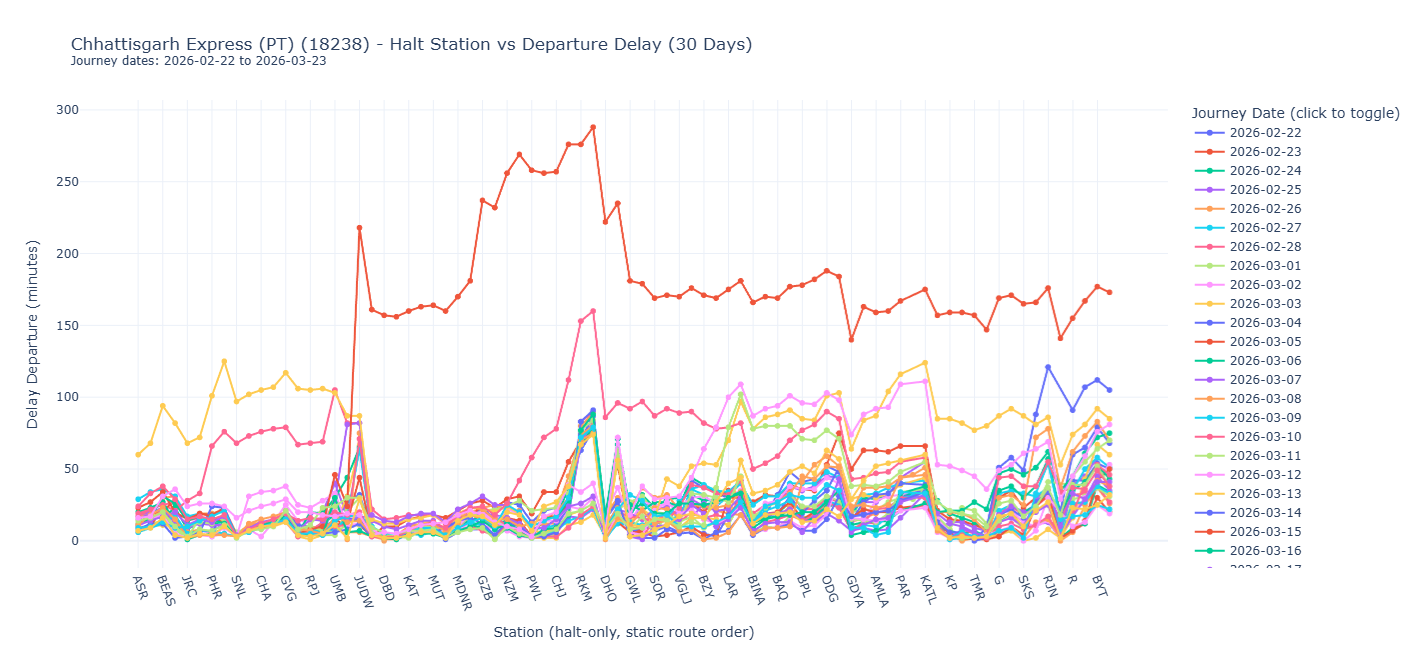
\includegraphics[width=1.12\textwidth]{../train_18238_station_delay_30d.png}
}{
    \fbox{\parbox{0.9\textwidth}{Placeholder: Train 18238 station vs departure delay plot (export from notebook)}}
}
\caption{Train 18238 (Chhattisgarh Express): halt-station vs departure delay pattern over the selected analysis window.}
\label{fig:train18238_delay}
\end{figure}

\section{Station-Pair Alpha Analysis}
To quantify station-segment behavior, we defined alpha on adjacent halt-station pairs for a journey:
\[
\alpha_{(i \rightarrow i+1)} = d_{i+1}^{(dep)} - d_i^{(dep)}
\]
where $d_i^{(dep)}$ is departure delay at station $i$.

\noindent Interpretation:
\begin{itemize}
    \item $\alpha > 0$: delay addition segment
    \item $\alpha < 0$: delay recovery (cover-up) segment
    \item practical threshold used: $|\alpha| \geq 1$ minute
\end{itemize}

Median alpha was used as the primary robust indicator and mean alpha as sensitivity check.

\subsection{Key Findings from Alpha Profiles}
Using the 30-day analysis window, the route does not follow one monotonic trend; it alternates between delay-add and recovery zones.

Examples observed in the notebook analysis include:
\begin{itemize}
    \item Strong delay-add segments: MTJ $\rightarrow$ RKM, BPHB $\rightarrow$ R, DHO $\rightarrow$ MRA
    \item Strong recovery segments: AGC $\rightarrow$ DHO, KATL $\rightarrow$ NGP, DUA $\rightarrow$ BINA
\end{itemize}

This supports the hypothesis that station/segment operational effects are persistent and measurable.

\begin{figure}[H]
\centering
\IfFileExists{../alpha_profile_plot.png}{
    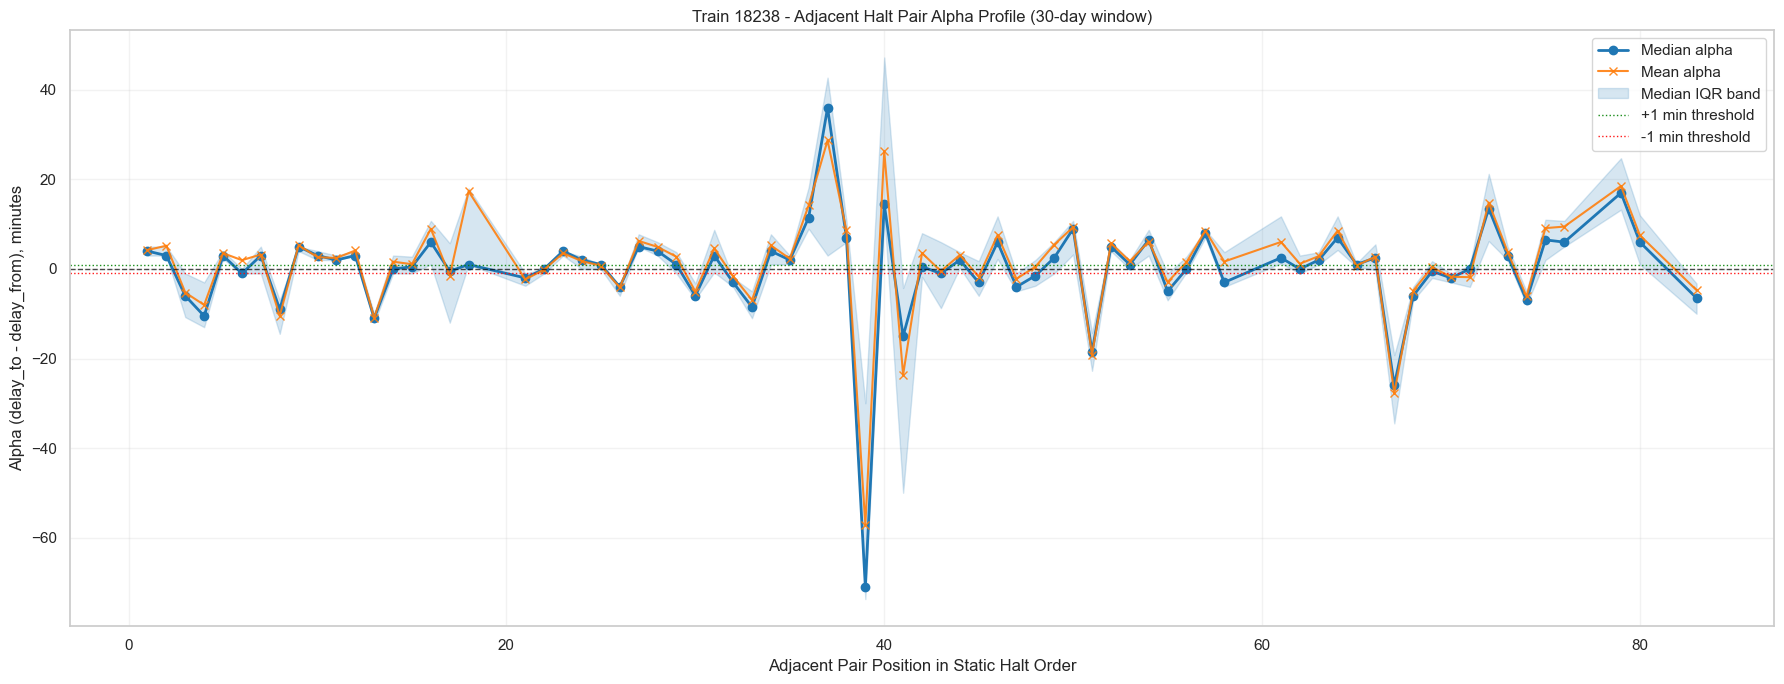
\includegraphics[width=1.1\textwidth]{../alpha_profile_plot.png}
}{
    \fbox{\parbox{0.9\textwidth}{Placeholder: Train 18238 alpha profile plot (median/mean with IQR band)}}
}
\caption{Train 18238 adjacent halt-pair alpha profile for the selected 30-day analysis window.}
\label{fig:alpha_profile_18238}
\end{figure}

\subsection{Top-10 Ranked Outputs (18238 Experiment)}
The experimentation stage reports ranked outputs for:
\begin{itemize}
    \item top-10 delay-adding pairs by median alpha,
    \item top-10 cover-up pairs by median alpha,
    \item top-10 delay-adding pairs by mean alpha,
    \item top-10 cover-up pairs by mean alpha,
    \item low-coverage pair diagnostics.
\end{itemize}
These rankings were generated in the notebook alpha analysis cells and are included in Appendix II for traceability.

\section{Baseline Modeling Status}
Baseline next-station delay prediction was performed for train 11077 using supervised models with journey-wise split to reduce leakage.

\begin{table}[H]
\centering
\caption{Baseline model metrics (current notebook run)}
\label{tab:model_metrics}
\begin{tabular}{lccc}
\toprule
Model & MAE (min) & RMSE (min) & MAPE (\%) \\
\midrule
Random Forest & 11.592 & 18.534 & $5.257897\times10^6$ \\
Polynomial Regression & 12.322 & 19.082 & $3.247892\times10^6$ \\
\bottomrule
\end{tabular}
\end{table}

\noindent The very high MAPE values indicate instability near zero-delay denominators and confirm that percentage-based error is not reliable for this target without additional handling.

\subsection{Time-Series Trials}
ARIMA/SARIMA/Prophet and Chronos baselines were explored, but initial outcomes were not adequate for the desired route-pattern capture. The current phase treats these as reference baselines, not final predictive claims.

\section{Limitations in Current Experimental Phase}
\begin{itemize}
    \item Selection bias can occur when severely delayed journeys cross abandonment thresholds.
    \item Coverage is currently limited to about three months of continuous data and 10 trains, so network-wide generalization is pending.
    \item Exogenous-factor comparison is currently limited: this phase did not observe strong seasonal extremes (for example, severe fog or monsoon rain), so weather-impact learning is weak in present baselines.
    \item Current experiments are primarily single-source and do not yet integrate richer factors such as weather feeds, infrastructure constraints, or control actions.
    \item Baseline models do not yet fully encode station-network structure.
\end{itemize}

% -------------------------
% CHAPTER 6
% -------------------------
\chapter{Conclusion and Future Work}

\section{Conclusion}
This minor project successfully established a data-centric pipeline for Indian Railways delay analytics and demonstrated that reliable station-level data generation is feasible with automated cloud workflows.

The project has produced:
\begin{itemize}
    \item a running collection infrastructure,
    \item a growing real-time dataset (40,000+ records),
    \item interpretable route-segment findings via alpha analysis,
    \item and reproducible baseline modeling benchmarks.
\end{itemize}

The core academic contribution of this phase is not a final high-accuracy predictor, but a robust and transparent data foundation plus interpretable diagnostics that make future modeling meaningful.

\section{Future Work}
Planned next steps are:
\begin{enumerate}
    \item advanced preprocessing and normalization of delay and time features,
    \item station-network aware feature engineering,
    \item graph-based representations for delay propagation,
    \item improved objective functions and robust metrics beyond MAPE,
    \item scaling train coverage and extending collection horizon.
\end{enumerate}

A promising direction is graph embedding based station-delay prediction as reported in recent literature; this aligns with our observation that delay behavior is strongly segment-dependent.

% -------------------------
% References
% -------------------------
\clearpage
\bibliographystyle{IEEEtran}
\bibliography{../references}

% -------------------------
% Appendices
% -------------------------
\appendix


\chapter{Experimental Figures and Alpha Tables}

\section*{A. Full Route-Ordered Alpha Table for Train 18238}
The following table is route-ordered and contains coverage ratio with both median and mean alpha values, corresponding to the notebook alpha experimentation output frame.

\small
\setlength{\LTleft}{0pt}
\setlength{\LTright}{0pt}
\begin{longtable}{r p{0.36\textwidth} r r r r}
\caption{Train 18238 route-ordered alpha table (median and mean with coverage ratio)}\label{tab:app_route_alpha_18238}\\
\toprule
Seq & Pair & $n$ & Coverage & Median $\alpha$ & Mean $\alpha$ \\
\midrule
\endfirsthead
\toprule
Seq & Pair & $n$ & Coverage & Median $\alpha$ & Mean $\alpha$ \\
\midrule
\endhead
\bottomrule
\endfoot
1 & ASR -> JNL & 30 & 1.000 & 4.000 & 4.233 \\
2 & JNL -> BEAS & 30 & 1.000 & 3.000 & 5.200 \\
3 & BEAS -> JUC & 30 & 1.000 & -6.000 & -5.267 \\
4 & JUC -> JRC & 30 & 1.000 & -10.500 & -8.033 \\
5 & JRC -> PGW & 30 & 1.000 & 3.000 & 3.533 \\
6 & PGW -> PHR & 30 & 1.000 & -1.000 & 1.967 \\
7 & PHR -> LDH & 30 & 1.000 & 3.000 & 3.233 \\
8 & LDH -> SNL & 30 & 1.000 & -9.000 & -10.500 \\
9 & SNL -> DOA & 30 & 1.000 & 5.000 & 5.300 \\
10 & DOA -> CHA & 30 & 1.000 & 3.000 & 2.633 \\
11 & CHA -> KNN & 30 & 1.000 & 2.000 & 2.467 \\
12 & KNN -> GVG & 30 & 1.000 & 3.000 & 4.133 \\
13 & GVG -> SIR & 30 & 1.000 & -11.000 & -10.900 \\
14 & SIR -> RPJ & 30 & 1.000 & 0.000 & 1.633 \\
15 & RPJ -> UBC & 30 & 1.000 & 0.500 & 1.067 \\
16 & UBC -> UMB & 30 & 1.000 & 6.000 & 8.967 \\
17 & UMB -> RAA & 30 & 1.000 & -0.500 & -1.500 \\
18 & RAA -> JUDW & 30 & 1.000 & 1.000 & 17.333 \\
21 & SRE -> DBD & 30 & 1.000 & -2.000 & -2.333 \\
22 & DBD -> MOZ & 30 & 1.000 & 0.000 & -0.133 \\
23 & MOZ -> KAT & 30 & 1.000 & 4.000 & 3.533 \\
24 & KAT -> DRLA & 30 & 1.000 & 2.000 & 1.733 \\
25 & DRLA -> MUT & 30 & 1.000 & 1.000 & 0.733 \\
26 & MUT -> MTC & 30 & 1.000 & -4.000 & -4.133 \\
27 & MTC -> MDNR & 30 & 1.000 & 5.000 & 6.267 \\
28 & MDNR -> GUH & 30 & 1.000 & 4.000 & 4.933 \\
29 & GUH -> GZB & 30 & 1.000 & 1.000 & 2.733 \\
30 & GZB -> SBB & 30 & 1.000 & -6.000 & -5.033 \\
31 & SBB -> NZM & 30 & 1.000 & 3.000 & 4.600 \\
32 & NZM -> BVH & 30 & 1.000 & -3.000 & -1.633 \\
33 & BVH -> PWL & 30 & 1.000 & -8.500 & -6.933 \\
34 & PWL -> KSV & 30 & 1.000 & 4.000 & 5.267 \\
35 & KSV -> CHJ & 30 & 1.000 & 2.000 & 2.300 \\
36 & CHJ -> MTJ & 30 & 1.000 & 11.500 & 14.200 \\
37 & MTJ -> RKM & 30 & 1.000 & 36.000 & 28.733 \\
38 & RKM -> AGC & 30 & 1.000 & 7.000 & 8.600 \\
39 & AGC -> DHO & 30 & 1.000 & -71.000 & -57.167 \\
40 & DHO -> MRA & 30 & 1.000 & 14.500 & 26.267 \\
41 & MRA -> GWL & 30 & 1.000 & -15.000 & -23.633 \\
42 & GWL -> DBA & 30 & 1.000 & 0.500 & 3.567 \\
43 & DBA -> SOR & 30 & 1.000 & -1.000 & -0.500 \\
44 & SOR -> DAA & 30 & 1.000 & 2.000 & 3.133 \\
45 & DAA -> VGLJ & 30 & 1.000 & -3.000 & -1.700 \\
46 & VGLJ -> BAB & 30 & 1.000 & 6.000 & 7.567 \\
47 & BAB -> BZY & 30 & 1.000 & -4.000 & -2.200 \\
48 & BZY -> TBT & 30 & 1.000 & -1.500 & 0.500 \\
49 & TBT -> LAR & 30 & 1.000 & 2.500 & 5.433 \\
50 & LAR -> DUA & 30 & 1.000 & 9.000 & 9.367 \\
51 & DUA -> BINA & 30 & 1.000 & -18.500 & -19.167 \\
52 & BINA -> MABA & 30 & 1.000 & 5.000 & 5.733 \\
53 & MABA -> BAQ & 30 & 1.000 & 1.000 & 1.733 \\
54 & BAQ -> BHS & 30 & 1.000 & 6.500 & 6.133 \\
55 & BHS -> BPL & 30 & 1.000 & -5.000 & -2.933 \\
56 & BPL -> RKMP & 30 & 1.000 & 0.000 & 1.533 \\
57 & RKMP -> ODG & 30 & 1.000 & 8.000 & 8.567 \\
58 & ODG -> NDPM & 30 & 1.000 & -3.000 & 1.667 \\
61 & GDYA -> BZU & 30 & 1.000 & 2.500 & 6.033 \\
62 & BZU -> AMLA & 30 & 1.000 & 0.000 & 1.167 \\
63 & AMLA -> MTY & 30 & 1.000 & 2.000 & 2.867 \\
64 & MTY -> PAR & 30 & 1.000 & 7.000 & 8.567 \\
65 & PAR -> NRKR & 4 & 0.133 & 1.000 & 0.750 \\
66 & NRKR -> KATL & 4 & 0.133 & 2.500 & 2.750 \\
67 & KATL -> NGP & 30 & 1.000 & -26.000 & -27.800 \\
68 & NGP -> KP & 30 & 1.000 & -6.000 & -4.867 \\
69 & KP -> BRD & 30 & 1.000 & -0.500 & 0.367 \\
70 & BRD -> TMR & 30 & 1.000 & -2.000 & -1.733 \\
71 & TMR -> TRO & 30 & 1.000 & 0.000 & -1.833 \\
72 & TRO -> G & 30 & 1.000 & 13.500 & 14.833 \\
73 & G -> AGN & 30 & 1.000 & 3.000 & 3.833 \\
74 & AGN -> SKS & 30 & 1.000 & -7.000 & -6.133 \\
75 & SKS -> DGG & 30 & 1.000 & 6.500 & 9.133 \\
76 & DGG -> RJN & 30 & 1.000 & 6.000 & 9.467 \\
79 & BPHB -> R & 26 & 0.867 & 17.000 & 18.538 \\
80 & R -> TLD & 29 & 0.967 & 6.000 & 7.517 \\
83 & BYT -> BYL & 30 & 1.000 & -6.500 & -4.733 \\
\end{longtable}

\section*{B. Top-10 Ranking Tables from Alpha Experimentation Phase}
These four ranking tables correspond to the top-10 outputs shown in the notebook alpha analysis (delay-adding and cover-up by median and mean alpha).

\begin{table}[H]
\centering
\small
\caption{Top-10 delay-adding pairs by median alpha (Train 18238)}
\label{tab:app_top10_median_add}
\begin{tabular}{p{0.27\textwidth} r r r r r}
\toprule
Pair & $n$ & Coverage & Median $\alpha$ & Mean $\alpha$ & IQR \\
\midrule
MTJ -> RKM & 30 & 1.000 & 36.000 & 28.733 & 39.750 \\
BPHB -> R & 26 & 0.867 & 17.000 & 18.538 & 11.500 \\
DHO -> MRA & 30 & 1.000 & 14.500 & 26.267 & 35.000 \\
TRO -> G & 30 & 1.000 & 13.500 & 14.833 & 15.000 \\
CHJ -> MTJ & 30 & 1.000 & 11.500 & 14.200 & 9.250 \\
LAR -> DUA & 30 & 1.000 & 9.000 & 9.367 & 7.500 \\
RKMP -> ODG & 30 & 1.000 & 8.000 & 8.567 & 1.750 \\
RKM -> AGC & 30 & 1.000 & 7.000 & 8.600 & 4.750 \\
MTY -> PAR & 30 & 1.000 & 7.000 & 8.567 & 7.500 \\
SKS -> DGG & 30 & 1.000 & 6.500 & 9.133 & 9.000 \\
\bottomrule
\end{tabular}
\end{table}

\begin{table}[H]
\centering
\small
\caption{Top-10 cover-up pairs by median alpha (Train 18238)}
\label{tab:app_top10_median_cover}
\begin{tabular}{p{0.27\textwidth} r r r r r}
\toprule
Pair & $n$ & Coverage & Median $\alpha$ & Mean $\alpha$ & IQR \\
\midrule
AGC -> DHO & 30 & 1.000 & -71.000 & -57.167 & 43.750 \\
KATL -> NGP & 30 & 1.000 & -26.000 & -27.800 & 15.250 \\
DUA -> BINA & 30 & 1.000 & -18.500 & -19.167 & 8.500 \\
MRA -> GWL & 30 & 1.000 & -15.000 & -23.633 & 45.750 \\
GVG -> SIR & 30 & 1.000 & -11.000 & -10.900 & 2.000 \\
JUC -> JRC & 30 & 1.000 & -10.500 & -8.033 & 10.000 \\
LDH -> SNL & 30 & 1.000 & -9.000 & -10.500 & 7.500 \\
BVH -> PWL & 30 & 1.000 & -8.500 & -6.933 & 6.000 \\
AGN -> SKS & 30 & 1.000 & -7.000 & -6.133 & 3.000 \\
BYT -> BYL & 30 & 1.000 & -6.500 & -4.733 & 6.750 \\
\bottomrule
\end{tabular}
\end{table}

\begin{table}[H]
\centering
\small
\caption{Top-10 delay-adding pairs by mean alpha (Train 18238)}
\label{tab:app_top10_mean_add}
\begin{tabular}{p{0.27\textwidth} r r r r r}
\toprule
Pair & $n$ & Coverage & Median $\alpha$ & Mean $\alpha$ & IQR \\
\midrule
MTJ -> RKM & 30 & 1.000 & 36.000 & 28.733 & 39.750 \\
DHO -> MRA & 30 & 1.000 & 14.500 & 26.267 & 35.000 \\
BPHB -> R & 26 & 0.867 & 17.000 & 18.538 & 11.500 \\
RAA -> JUDW & 30 & 1.000 & 1.000 & 17.333 & 17.000 \\
TRO -> G & 30 & 1.000 & 13.500 & 14.833 & 15.000 \\
CHJ -> MTJ & 30 & 1.000 & 11.500 & 14.200 & 9.250 \\
DGG -> RJN & 30 & 1.000 & 6.000 & 9.467 & 5.750 \\
LAR -> DUA & 30 & 1.000 & 9.000 & 9.367 & 7.500 \\
SKS -> DGG & 30 & 1.000 & 6.500 & 9.133 & 9.000 \\
UBC -> UMB & 30 & 1.000 & 6.000 & 8.967 & 9.750 \\
\bottomrule
\end{tabular}
\end{table}

\begin{table}[H]
\centering
\small
\caption{Top-10 cover-up pairs by mean alpha (Train 18238)}
\label{tab:app_top10_mean_cover}
\begin{tabular}{p{0.27\textwidth} r r r r r}
\toprule
Pair & $n$ & Coverage & Median $\alpha$ & Mean $\alpha$ & IQR \\
\midrule
AGC -> DHO & 30 & 1.000 & -71.000 & -57.167 & 43.750 \\
KATL -> NGP & 30 & 1.000 & -26.000 & -27.800 & 15.250 \\
MRA -> GWL & 30 & 1.000 & -15.000 & -23.633 & 45.750 \\
DUA -> BINA & 30 & 1.000 & -18.500 & -19.167 & 8.500 \\
GVG -> SIR & 30 & 1.000 & -11.000 & -10.900 & 2.000 \\
LDH -> SNL & 30 & 1.000 & -9.000 & -10.500 & 7.500 \\
JUC -> JRC & 30 & 1.000 & -10.500 & -8.033 & 10.000 \\
BVH -> PWL & 30 & 1.000 & -8.500 & -6.933 & 6.000 \\
AGN -> SKS & 30 & 1.000 & -7.000 & -6.133 & 3.000 \\
BEAS -> JUC & 30 & 1.000 & -6.000 & -5.267 & 9.750 \\
\bottomrule
\end{tabular}
\end{table}

\section*{C. Low-Coverage Diagnostic Note}
Low-coverage pairs in the notebook output were mainly concentrated around sparse route segments (for example PAR$\rightarrow$NRKR and NRKR$\rightarrow$KATL), while several downstream pairs had no observations in the selected 30-day window. These should be treated as provisional until additional journey data is collected.

\section*{D. Placeholder Space for Nine Station-vs-Delay Train Plots}
Main chapter already includes Train 18238. The following space is reserved for the remaining nine train plots.
\begin{figure}[H]
\centering
\fbox{\parbox{0.9\textwidth}{\vspace{8cm}\centering Reserved space for nine station-vs-departure-delay plots\vspace{8cm}}}
\caption{Reserved space for nine additional station-vs-delay plots.}
\end{figure}

\end{document}
